\chapter{Results}\label{chapter:results}

To search for and quantify the significance of the production of signals $\left(V, H, \Zprime\right)$, and to set limits in the absence of observation, a Bayesian method is used to calculate a posterior likelihood as a function of number of signal events for the signal hypotheses under consideration~\cite{EXOT-2010-07}.
In this method, a final conditional probability of the parameters of interest given the observed data (the ``posterior'') is built by integrating over the nuisance parameters (``marginalization'') with a Markov Chain Monte Carlo (\Gls{MCMC}) procedure.
The posterior distribution is used to gauge the fitted signal statistical significance or to set $95\%$ credibility-level upper limits on the cross-section times acceptance times efficiency.

\section{Measurement of Standard Model Signals}

To measure the Standard Model signals a model comprised of the Standard Model $\Vjets$, $\Hbb$, and $\ttbar$ signal templates along with the QCD multijet model is fit to the data.
The normalization of the $\ttbar$ component of the model is constrained with the scale factor obtained in the dedicated $\ttbar$ Control Region.
This fit simultaneously extracts the signal strengths of the $\Vjets$ and $\Hbb$ process, $\mu_{V}$ and $\mu_{H}$ respectively, which are unconstrained.
The comparison of the model post marginalization of the nuisance parameters to the data is seen in Figure~\ref{fig:post_fit}.

\begin{figure}[htbp]
 \centering
 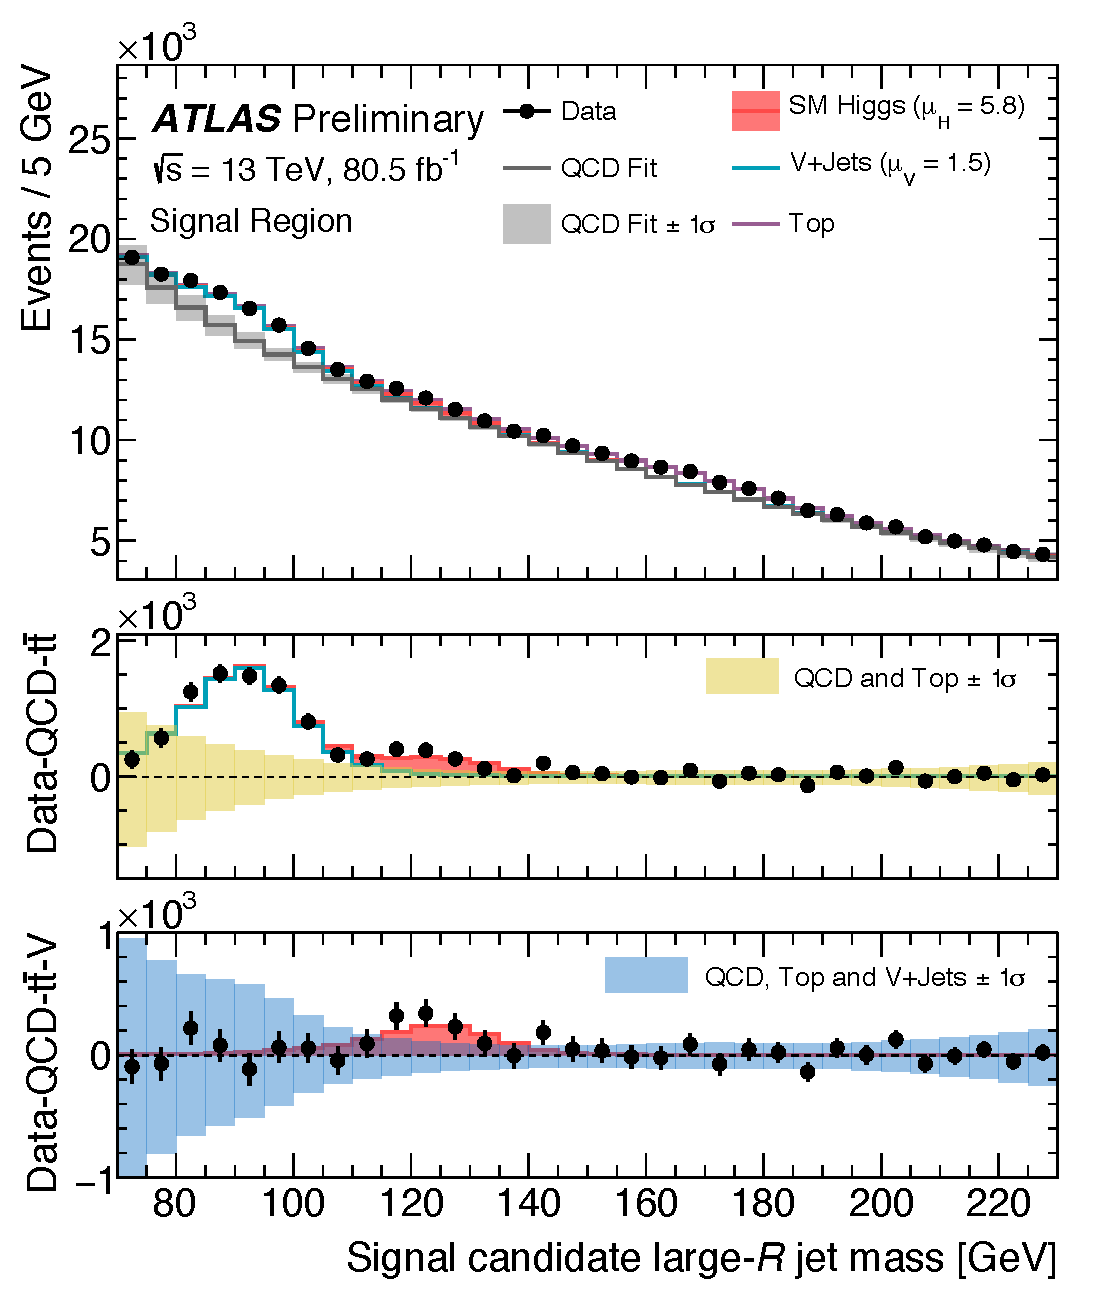
\includegraphics[width=\linewidth]{results/SRPostFit_mass}
 \caption{The top panel shows the post fit plot of the SM Higgs boson, $\Vjets$, $\ttbar$ and QCD model with the observed data.
  The middle panel shows the post fit model and the data with the QCD and $\ttbar$ components of the model subtracted, highlighting the large resonance from $\Vjets$.
  The bottom panel shows the post fit model and the data with the QCD, $\Vjets$, and $\ttbar$ components of the model subtracted, highlighting a small excess of events near $125~\GeV$.
 }
 \label{fig:post_fit}
\end{figure}

\subsection{Observation of boosted $V\to b\bar{b}$}

The observed signal strength for the $\Vjets$ process is\\ $\mu_{V} = 1.5 \pm 0.22~\mathrm{(stat.)}^{+0.29}_{-0.25}~\mathrm{(syst.)} \pm 0.18~\mathrm{(th.)}$, corresponding to an observed significance of $5\,\sigma$ with an expected significance of $4.8\,\sigma$.
This constituents the first direct observation of boosted vector bosons decaying to bottom quark pairs in ATLAS.\footnote{\TODO{} Double verify this.}

\subsection{Measurement of boosted $H\to b\bar{b}$}
For the $\Hbb$ process, the observed signal strength is\\ $\mu_{H} = 5.8 \pm 3.1~\mathrm{(stat.)} \pm 1.9~\mathrm{(syst.)} \pm 1.7~\mathrm{(th.)}$, which given the uncertainties is consistent with the background-only hypothesis at $1.6\,\sigma$ with an expected sensitivity of $0.28\,\sigma$.
This constituents a measurement of boosted Higgs decaying to bottom quark pairs, though not a direct observation.

The combined posterior distributions of $\mu_{V}$ and $\mu_{H}$ is seen in Figure~\ref{fig:signal_strength_contour}, showing the agreement between the best fit values of the model and the Standard Model prediction of $\mu_{V} = \mu_{H} = 1$.

\begin{figure}[htbp]
 \centering
 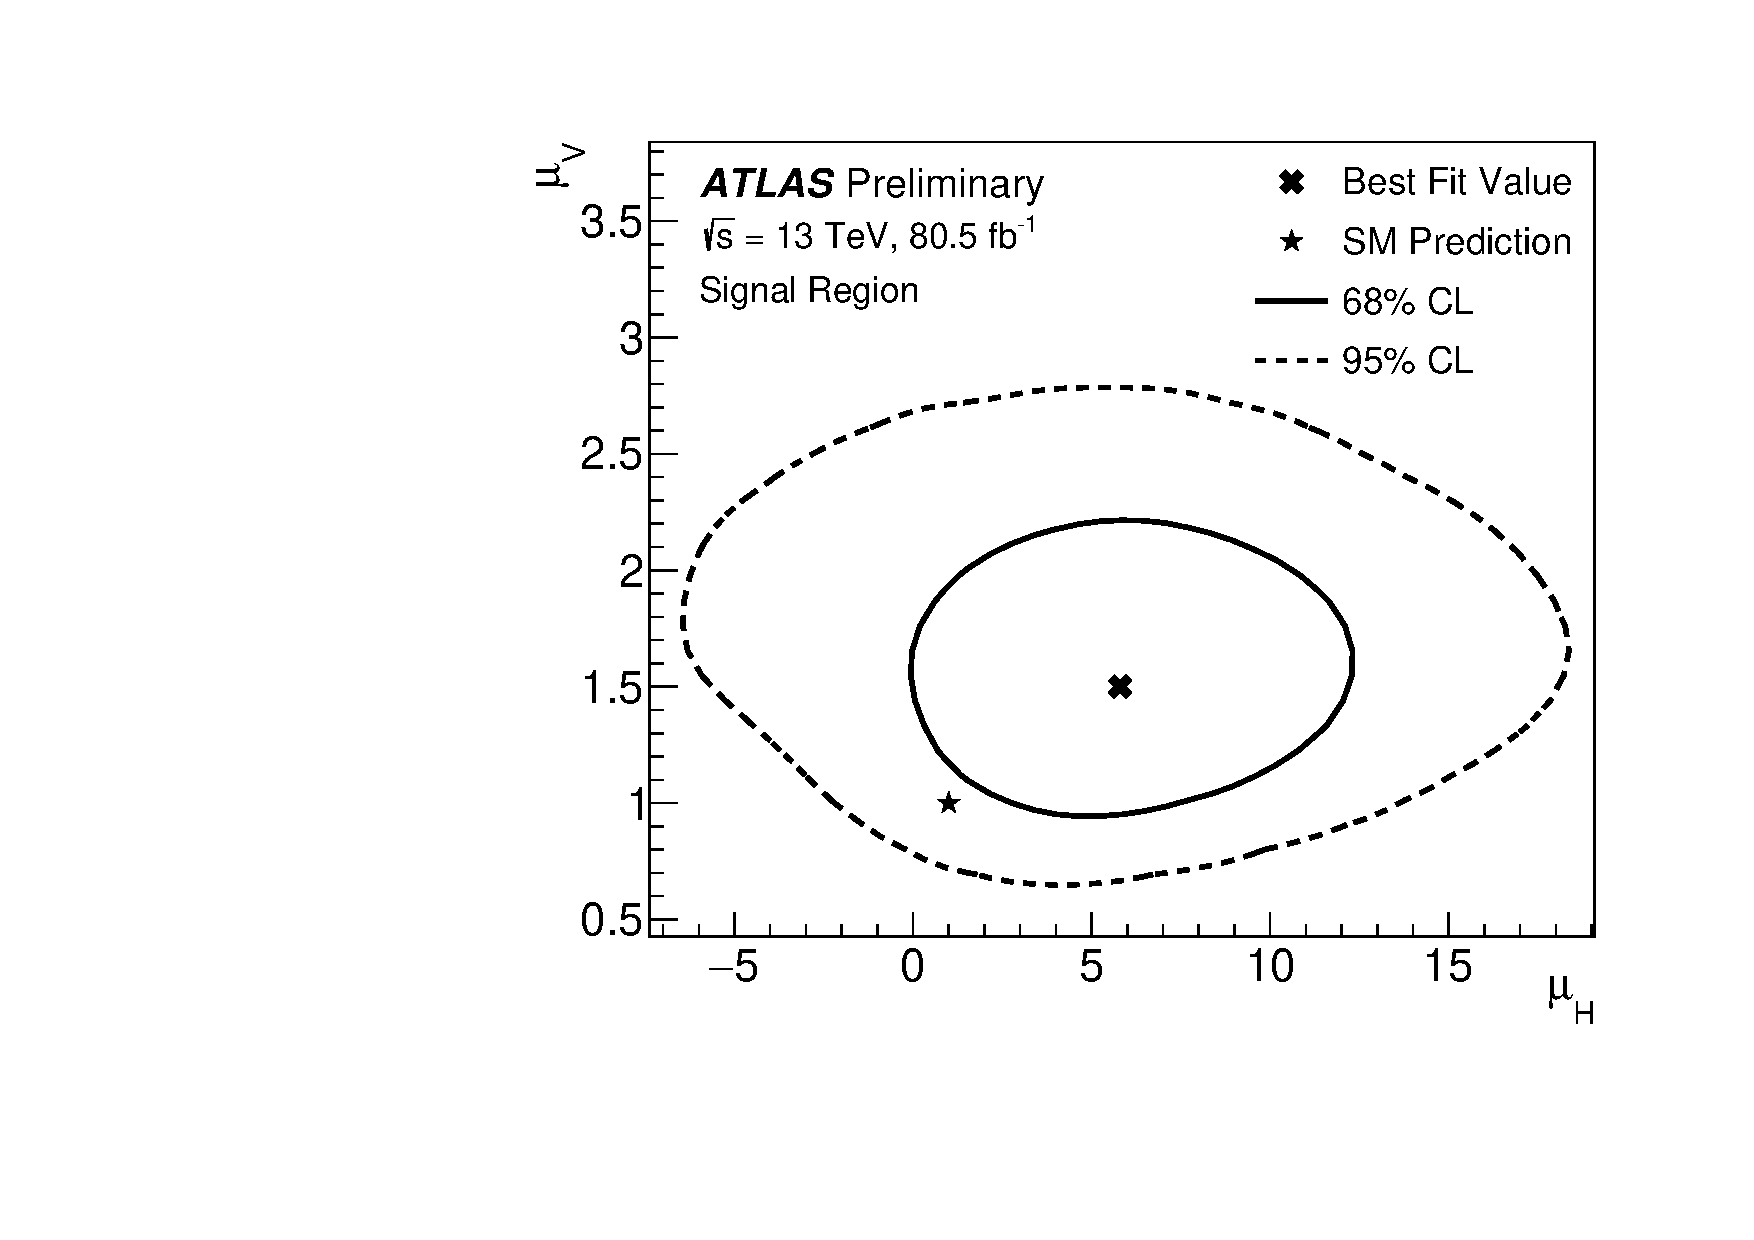
\includegraphics[width=0.6\linewidth]{results/contourFinal}
 \caption{Combined posterior distributions of $\mu_{H}$ and $\mu_{V}$ from the signal region fit.
  It is seen that the best fit values for the signal processes lie within the $2\,\sigma$ interval of the Standard Model prediction.}
 \label{fig:signal_strength_contour}
\end{figure}

\section{Limits on $\Zprime$ production}

Following the measurement of the Standard Model signals, a search for exotic signals in the \largeR jet mass distribution is performed.
The first step in the search is to apply the \BumpHunter{} search procedure \cite{Aaltonen:2008vt,Choudalakis:2011qn}.
Given that the effect of the Higgs boson with a SM strength is smaller than the expected uncertainty on the $\Zprime$ limit the SM Higgs template is excluded from the model, and only the $\Vjets$ and $\ttbar$ templates are considered along with the QCD parametric model.
With this model, a fit to the data is performed with the full set of systematic uncertainties resulting in the best fit values for the model nuisance parameters used in the analysis.
With these post fit shapes, the \BumpHunter{} algorithm scans the mass range looking for significant deviations from the background-only model.
For the given model, the largest deviation from the background is found in the \largeR jet mass interval of $\left[115,130\right]~\GeV$, as seen in Figure~\ref{fig:BumpHunter_scan}.
This deviation has a \BumpHunter{} global $p$-value\footnote{\TODO{} Explain how this \BumpHunter{} $p$-value is calculated.} of $0.54$, indicating that the model is quite consistent with the data.\\

\begin{figure}[htbp]
 \centering
 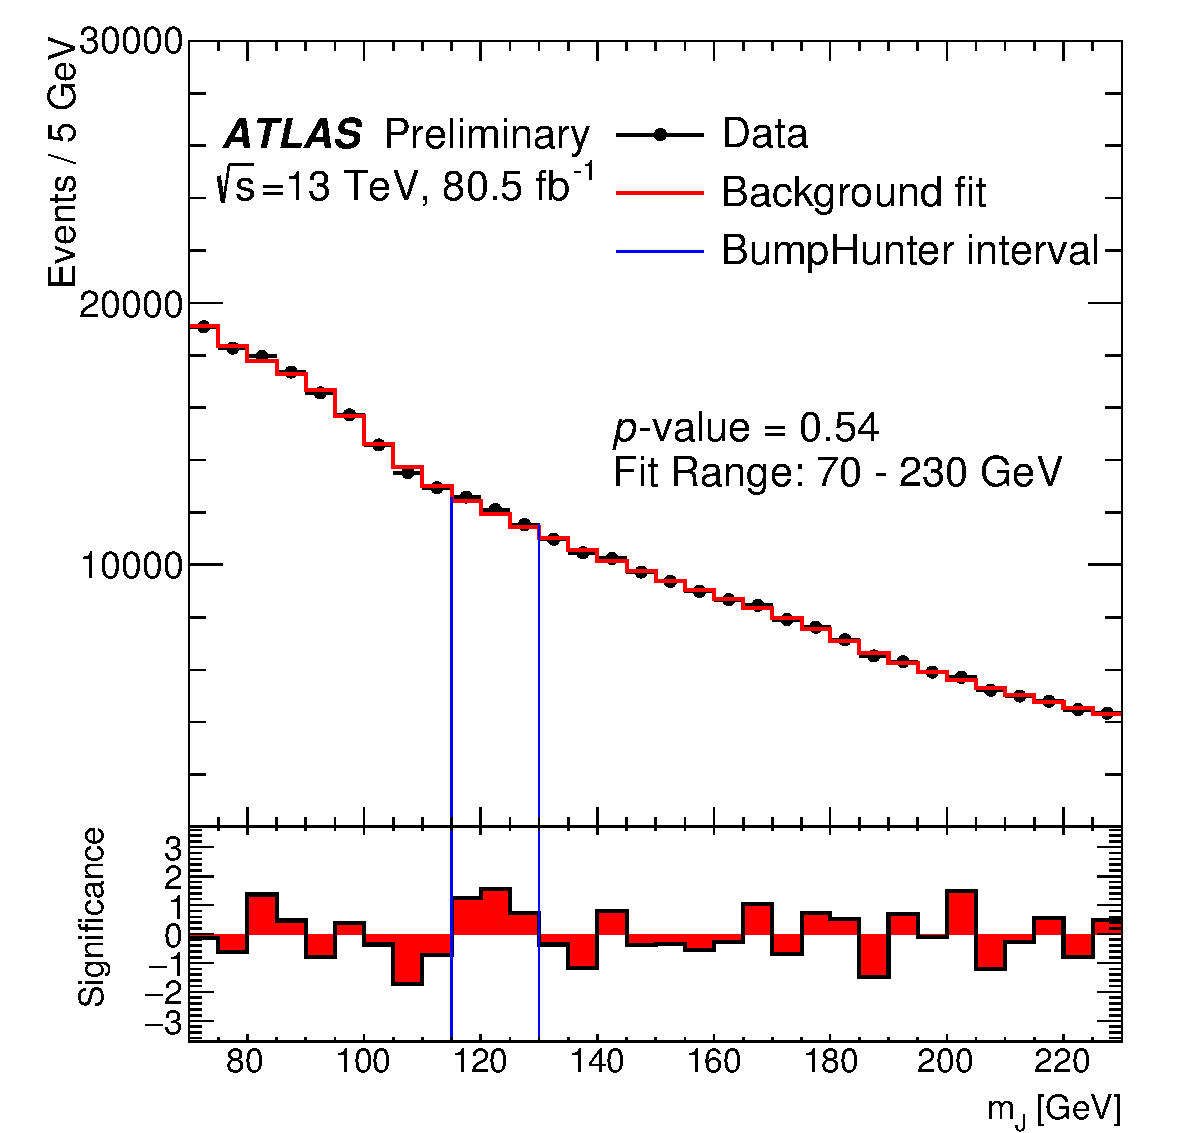
\includegraphics[width=\linewidth]{results/BH_final}
 \caption{The reconstructed mass distribution $m_{J}$ with the event reconstruction and selection as described in the text.
  The solid red line depicts the background prediction, consisting of the non-resonant dijet, $\Vjets$, and $\ttbar$ processes.
  The vertical blue lines indicate the most discrepant interval identified by the \BumpHunter{} algorithm between $115~\GeV$ and $130~\GeV$.
  Without including systematic uncertainties, the probability that fluctuations of the background model would produce an excess at least as significant as the one observed in the data anywhere in the distribution, the \BumpHunter{} probability, is $0.54$.
  The bottom panel shows the bin-by-bin significances \textbf{\TODO{} State how these significances are defined} of the differences between the data and the fit, considering only statistical fluctuations.
 }
 \label{fig:BumpHunter_scan}
\end{figure}

In the absence of excesses in the data that could correspond to new physics, $95\%$ confidence level limits are set on signals from dark matter mediators with democratic decays to quarks with masses between $100~\GeV$ and $200~\GeV$.
These limits are shown in Figure~\ref{fig:Zprime_limits}, in terms of cross section times branching ratio, acceptance and efficiency (Figure~\ref{fig:cross_section_limits}), and in terms of the $g_{q}$ parameter that controls the coupling of the \gls{dark matter mediator} to quarks that determines the cross-section (Figure~\ref{fig:gq_limits}).
From these limits, an exotic dark matter mediator $\Zprime$ with $g_{q}=0.25$ is excluded for $m_{\Zprime} < 200~\GeV$ at the $95\%~\mathrm{CL}$.

\begin{figure}[htbp]
 \centering
 \begin{subfigure}[t]{0.5\textwidth}
  \centering
  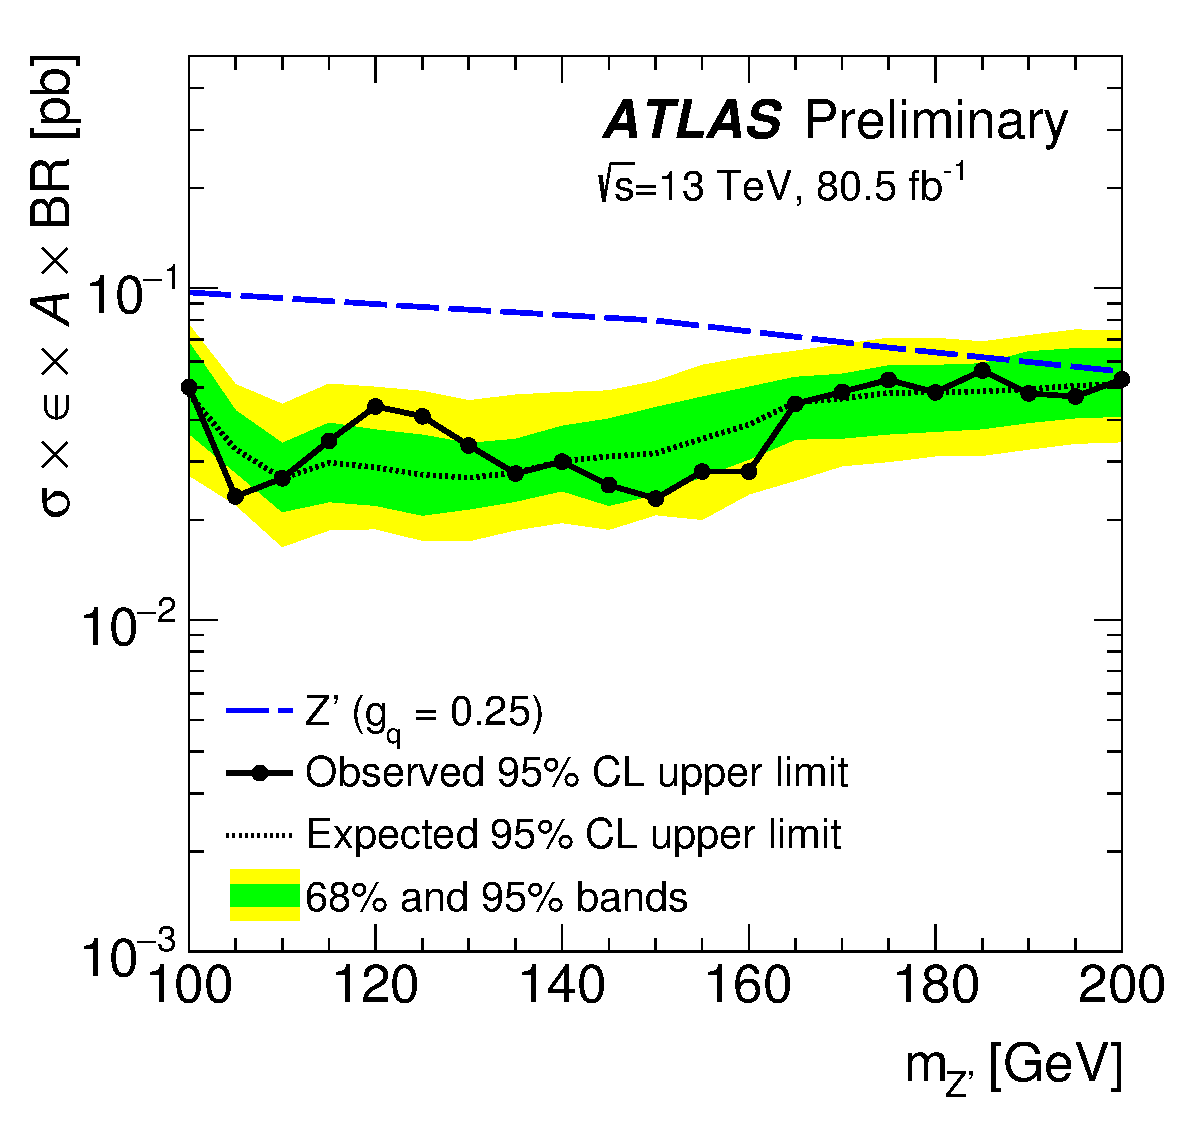
\includegraphics[width=\textwidth]{results/Final_Limits}
  \caption{The limit on the cross-section times acceptance times branching ratio times efficiency.}
  \label{fig:cross_section_limits}
 \end{subfigure}%
 ~
 \begin{subfigure}[t]{0.5\textwidth}
  \centering
  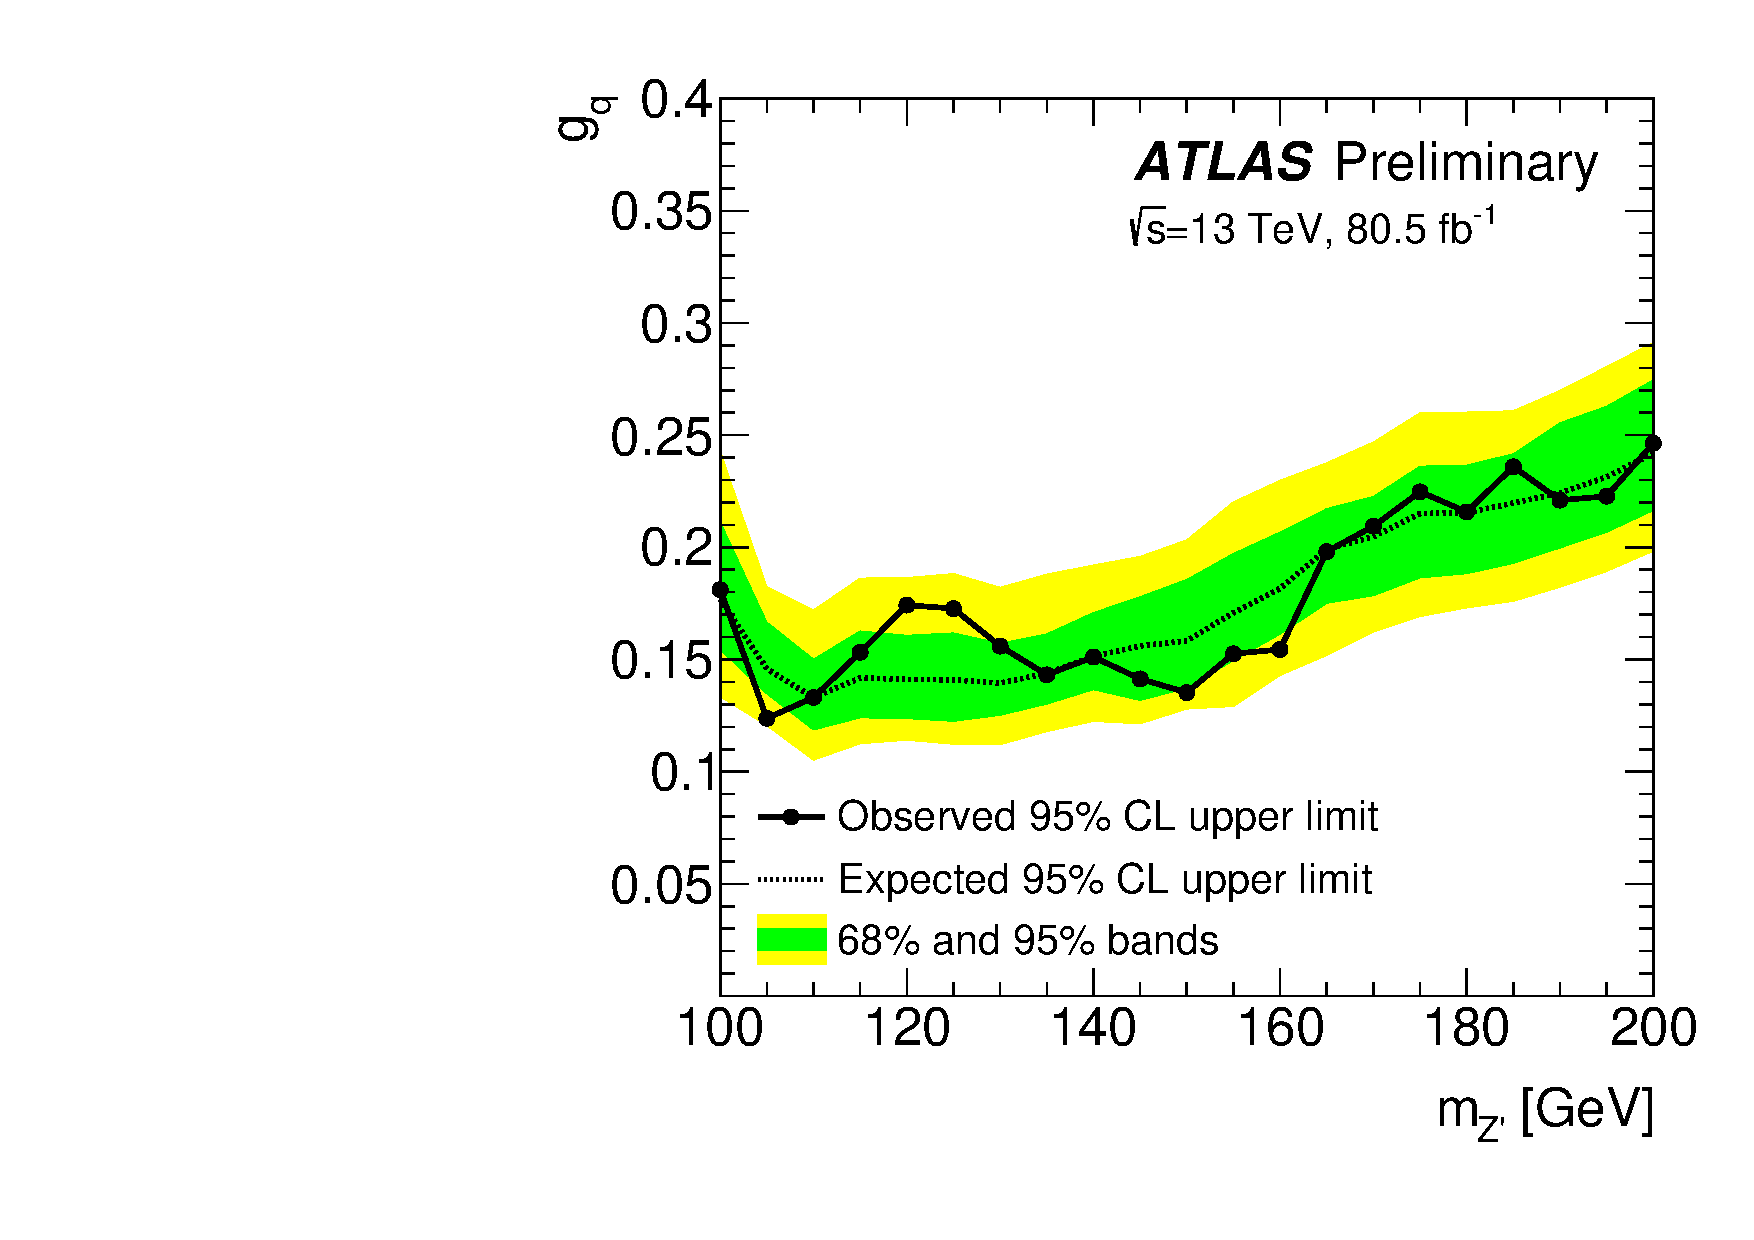
\includegraphics[width=\textwidth]{results/gqlimit}
  \caption{The limit on the $g_{q}$ parameter that controls the decay width of the $\Zprime$ into SM quarks.}
  \label{fig:gq_limits}
 \end{subfigure}
 \caption{The $95\%$ credibility-level upper limits obtained from the invariant mass distribution for the $\Zprime$ dark matter mediator model.}
 \label{fig:Zprime_limits}
\end{figure}
